\documentclass{beamer}
\usetheme{simple}
\usepackage[brazil]{babel}
\usepackage[utf8]{inputenc}
\usepackage{lmodern} 
\usefonttheme[onlymath]{serif}
\usepackage[scale=2]{ccicons} 

\usepackage{graphicx,hyperref,url,pgfplots}
\usepackage{media9}
\usepackage{amsmath} 
\usepackage{array,booktabs}
\usepackage{pdfpages}
\pgfplotsset{compat=1.13}  
\pgfplotsset{width=7cm}


\setbeamercovered{invisible} 
\newcommand{\pausar}{\pause}
\newcommand{\df}[1]{\,\mathrm{d}#1}
\newcommand{\parcial}[3]{\dfrac{\partial^{#1}#2}{\partial #3^{#1}}}

\usepackage{tikz}
\usepackage{xcolor}
\usetikzlibrary{scopes}
\usepackage{verbatim}
\usetikzlibrary{patterns}
\usepackage{algorithm}
\usepackage{algpseudocode}

\usepackage{listings}
	\definecolor{codegreen}{rgb}{0,0.6,0}
	\definecolor{codegray}{rgb}{0.5,0.5,0.5}
	\definecolor{codepurple}{rgb}{0.58,0,0.82}
	\definecolor{backcolour}{rgb}{0.92,0.92,0.92}
	\lstset{language=Python, 
	backgroundcolor=\color{backcolour},   
	commentstyle=\color{codegreen},
	keywordstyle=\color{magenta},
	numberstyle=\tiny\color{codegray},
	stringstyle=\color{codepurple},
	basicstyle=\fontsize{8}{11}\ttfamily,
	frame=lines,
%	numbers=left,
	tabsize=2,
	morekeywords={models, lambda, forms}}


\title{Filtro de Kalman}
\subtitle{Aplicações na Robótica Móvel}
\date{\today}
\author{Jeferson Lima}
\institute{\url{http://gitlab.com/jeferson.lima}}

\begin{document}

\maketitle

% \begin{frame}{Informações Úteis}
% 	\begin{block}{Material disponível em:}
% 		\href{Robótica Móvel - Wiki}{https://gitlab.com/cursoseaulas/robotica-movel/-/wikis/home}
% 	\end{block}
% 	\pausar
% 	\begin{block}{Datas Importantes}
% 		\begin{itemize}
% 		\item Entrega
% 		\item Envio
% 		\end{itemize}
% 	\end{block}
% 	\pausar
% 	\begin{block}{Requisitos da Disciplina}
% 		\begin{itemize}
% 		\item Teoria de Controle
% 		\item Linguagem de Programação - \textbf{Python} ou \textbf{C++}
% 		\item Eletrônica
% 		\end{itemize}
% 	\end{block}
% \end{frame}

%-----------------------------------------------------------------

\begin{frame}{Teorema de Bayes}
    \framesubtitle{Revisão} {Revisão}
  \begin{itemize}
    \item Estado Estimado $x$ de um sistema observado $z$ e com controle em $u$.
    \item Objetivo:
  \end{itemize}

  \begin{equation}
    P(x|z,u)
  \end{equation}
\end{frame}


\begin{frame}{Bayes Filter}
    \framesubtitle{Revisão}
    
    \begin{block}{}
        \begin{equation*}
            \text{Bel}(x_t) = \eta P(z_t| x_t) \int P(x_t| u_t, x_{t-1}) \text{Bel}(x_{t-1})\text{d}x_{t-1}
        \end{equation*}
    \end{block}

    \begin{itemize}
        \item Predição:
        
        \begin{equation*}
            \overline{\text{Bel}}(x_t) = \int P(x_t| u_t, x_{t-1}) \text{Bel}(x_{t-1})\text{d}x_{t-1}
        \end{equation*}

        \item Correção:

        \begin{equation*}
            \text{Bel}(x_t) = \eta P(z_t| x_t) \int P(x_t| u_t, x_{t}) \overline{\text{Bel}}(x_{t})\text{d}x_{t-1}
        \end{equation*}
    \end{itemize}
\end{frame}


\begin{frame}{Distribuição Normal (Gaussiana)}
    \framesubtitle{Revisão}  
    \begin{itemize}
        \item \textbf{Uma Variável:} $\color{blue}{P(x) \sim N(\mu, \sigma^2)}$
    \end{itemize}
    \begin{block}{}
        \begin{equation*}
            P(x) = \dfrac{1}{\sqrt{2\pi\sigma^2}}\cdot 
        \exp\left\{-\frac{(x-\mu)^2}{2\sigma^2}\right\}
        \end{equation*}
    \end{block}
    \centering
    \begin{tikzpicture}[
    declare function={
      normalpdf(\x,\mu,\sigma)=
      (2*3.1415*\sigma^2)^(-0.5)*exp(-(\x-\mu)^2/(2*\sigma^2));
    },
    hplot/.style={ycomb, mark=o, dashed}, ,scale=0.8]
  
    \begin{axis}[
      width=12cm, height=6cm,
      samples=50,
      xlabel=$x$, ylabel=$p(x)$,
      xlabel style={at={(1,0)}, anchor=north west},
      ylabel style={rotate=-90, at={(0,1)}, anchor=south east},
      legend style={draw=none, fill=none},
      domain=-6:9,
      legend cell align=left,
      xmin=-7, xmax=11]
  
      \addplot [smooth, thick] {normalpdf(x,0,1)}
      node[pos=0.47, pin={right:$\mu=0,\sigma^2=1$}] {};
      \addplot [smooth, blue] {normalpdf(x,0,2)}
      node[pos=0.6, pin={45:$\mu=0,\sigma^2=2$}] {};
      \addplot [smooth, red] {normalpdf(x,-2,1)}
      node[pos=0.25, pin={[text centered, text width=8ex]
        200:$\mu=-1$, $\sigma^2=1$}] {};
  
      \addplot [hplot, samples at={0}] {normalpdf(x,0,1)};
      \addplot [hplot, samples at={0}, blue] {normalpdf(x,0,2)};
      \addplot [hplot, samples at={-2}, red] {normalpdf(x,-2,1)};
  
      \node[anchor=north east] at (axis description cs: 0.975,  0.95)
      {$p(x) = \dfrac{1}{\sqrt{2\pi\sigma^2}}\cdot 
        \exp\left\{-\frac{(x-\mu)^2}{2\sigma^2}\right\}$};
  
    \end{axis}
  \end{tikzpicture}
\end{frame}


\begin{frame}{Distribuição Normal (Gaussiana)}
    \framesubtitle{Revisão}
    \begin{itemize}
        \item Bivariável: $\color{blue}{P(\mathbf{x}) \sim N(\mu, \textstyle\sum)}$
    \end{itemize}
    \centering
    \resizebox{0.6\textwidth}{!}{
\pgfplotsset{%
  colormap={whitered}{color(0cm)=(white);
  color(1cm)=(orange!75!red)}
}
\begin{tikzpicture}[
  declare function = {mu1=1;},
  declare function = {mu2=2;},
  declare function = {sigma1=0.5;},
  declare function = {sigma2=1;},
  declare function = {normal(\m,\s)=1/(2*\s*sqrt(pi))*exp(-(x-\m)^2/(2*\s^2));},
  declare function = {bivar(\ma,\sa,\mb,\sb)=
    1/(2*pi*\sa*\sb) * exp(-((x-\ma)^2/\sa^2 + (y-\mb)^2/\sb^2))/2;},scale=0.6]
  \begin{axis}[
    colormap name  = whitered,
    width          = 15cm,
    view           = {45}{65},
    enlargelimits  = false,
    grid           = major,
    domain         = -1:4,
    y domain       = -1:4,
    samples        = 26,
    xlabel         = $x_1$,
    ylabel         = $x_2$,
    zlabel         = {$P$},
    colorbar,
    colorbar style = {
      at     = {(1,0)},
      anchor = south west,
      height = 0.25*\pgfkeysvalueof{/pgfplots/parent axis height},
      title  = {$P(x_1,x_2)$}
    }
  ]
    \addplot3 [surf] {bivar(mu1,sigma1,mu2,sigma2)};
    \addplot3 [domain=-1:4,samples=31, samples y=0, thick, smooth]
      (x,4,{normal(mu1,sigma1)});
    \addplot3 [domain=-1:4,samples=31, samples y=0, thick, smooth]
      (-1,x,{normal(mu2,sigma2)});

    \draw [black!50] (axis cs:-1,0,0) -- (axis cs:4,0,0);
    \draw [black!50] (axis cs:0,-1,0) -- (axis cs:0,4,0);

    \node at (axis cs:-1,1,0.18) [pin=165:$P(x_1)$] {};
    \node at (axis cs:1.5,4,0.32) [pin=-15:$P(x_2)$] {};
  \end{axis}
\end{tikzpicture}}
\end{frame}



\begin{frame}{Distribuição Normal (Gaussiana)}
    \framesubtitle{Revisão}
    \begin{itemize}
        \item Bivariável: $\color{blue}{p(\mathbf{x}) \sim N(\mu, \textstyle\sum)}$
    \begin{equation*}
        P(\mathbf{x}) = \frac{1}{(2\pi)^{\frac{d}{2}\|\textstyle\sum\|^{\frac{1}{2}}}}\exp\left\{-\frac{1}{2} (\mathbf{x}-\mu)^T\textstyle\sum{}^{-1}(\mathbf{x}-\mu)\right\}
    \end{equation*}
    
    \item Para um sistema de duas Variável:
    
    \begin{equation*}
        p(\mathbf{x}) \sim N(\mu, \textstyle\sum)
    \end{equation*}
    logo:     
    \begin{equation*}
        \begin{pmatrix}
            X_1 \\
            X_2
        \end{pmatrix}  \sim \mathcal{N} \left( \begin{pmatrix}
            \mu_1 \\
            \mu_2
        \end{pmatrix} , \begin{pmatrix}
            \sigma^2_1 &  \rho \sigma_1 \sigma_2 \\
            \rho \sigma_1 \sigma_2 &  \sigma^2_2
        \end{pmatrix} \right)
    \end{equation*}
    \end{itemize}
\end{frame}

\begin{frame}{Distribuição Normal (Gaussiana)}
    \framesubtitle{Propriedades}
    \begin{itemize}
        \item Caso Univariavel:
        \begin{equation}
            \left.
            \begin{aligned}
                    X & \sim N\left(\mu, \sigma_2\right)\\
                    Y & = aX + b\\
            \end{aligned} \right\}
            \quad \Rightarrow \quad Y \sim N\left(a\mu+b\right)
        \end{equation}
        \item Caso Multivariável:
        \begin{equation}
            \left.
            \begin{aligned}
                    X & \sim N\left(\mu, \textstyle\sum\right)\\
                    Y & = AX + B\\
            \end{aligned} \right\}
            \quad \Rightarrow \quad Y \sim N\left( A\mu+B, A\textstyle\sum A^T \right)
        \end{equation}
    \end{itemize}
\end{frame}


\begin{frame}{Kalman filter}
    \framesubtitle{Modelo determinístico e estocástico}
    \begin{itemize}
        \item Num \textcolor{blue}{modelo determinístico} o resultado do sistema é pré determinado em função dos dados de entrada, exemplo:
        \begin{align*} 
            x_t &= A_t x_{t-1} + B_t u_t\\ 
            z_t &= C_t x_t
        \end{align*}
        \item Num \textcolor{blue}{modelo estocástico} o resultado do sistema não depende somente dos dados de entrada, mas também de outros fatores, normalmente
        aleatórios:
        \begin{align} 
            x_t &= A_t x_{t-1} + B u_t +  w_t\\ 
            z_t &= C_t x_t + v_t
        \end{align}
        \begin{itemize}
            \item $A_t$ Matriz $(n \times n)$ que descreve os estados do modelo.
            \item $B_t$ Matriz $(n \times l)$ que descreve os estados do controle.
            \item $C_t$ Matrix $(k\times n)$ sendo os estados de $x_t$.
            \item $ w_t$ Variável aleatória do processo com distribuição normal e covariância $Q_t$.
            \item $v_t$ Rúido aleatório com distribuição normal e covariância de $R_t$.
        \end{itemize}
    \end{itemize}
\end{frame}


\begin{frame}{Kalman filter}
    \framesubtitle{Representação Grafica}
      \begin{tikzpicture}[
    declare function={
      normalpdf(\x,\mu,\sigma)=
      (2*3.1415*\sigma^2)^(-0.5)*exp(-(\x-\mu)^2/(2*\sigma^2));
    },
    hplot/.style={ycomb, mark=o, dashed}, ,scale=0.8]
  
    \begin{axis}[
      width=10cm, height=5.5cm,
      samples=50,
      legend style={draw=none, fill=none},
      domain=-6:9,
      legend cell align=left,
      xmin=-7, xmax=11]
  
      \addplot [smooth, thick, red] {normalpdf(x,-2,2)} node[] {};
      \addplot [dashed, gray]       {normalpdf(x,-5,1.5)} node[] {};
      \legend{Motion Model, $\text{Bel}(x_{t-1})$};
    \end{axis}
  \end{tikzpicture}
  \pausar
  \begin{tikzpicture}[
    declare function={
      normalpdf(\x,\mu,\sigma)=
      (2*3.1415*\sigma^2)^(-0.5)*exp(-(\x-\mu)^2/(2*\sigma^2));
    },
    hplot/.style={ycomb, mark=o, dashed}, ,scale=0.8]
  
    \begin{axis}[
      width=10cm, height=5.5cm,
      samples=50,
      legend style={draw=none, fill=none},
      domain=-6:9,
      legend cell align=left,
      xmin=-7, xmax=11]
  
      \addplot [smooth, thick, red] {normalpdf(x,-2,2)} node[] {};
      \addplot [smooth, black] {normalpdf(x,0,2)} node[] {};
      \addplot [dashed, gray]       {normalpdf(x,-5,1.5)} node[] {};
      \legend{Motion Model, sensor $z_i$, $\text{Bel}(x_{t-1})$};
    \end{axis}
  \end{tikzpicture}

  \pausar

\begin{columns}

  \begin{column}{0.5\textwidth}

    \begin{tikzpicture}[
      declare function={
        normalpdf(\x,\mu,\sigma)=
        (2*3.1415*\sigma^2)^(-0.5)*exp(-(\x-\mu)^2/(2*\sigma^2));
      },
      hplot/.style={ycomb, mark=o, dashed}, ,scale=0.8]
    
      \begin{axis}[
        width=10cm, height=5.5cm,
        samples=50,
        legend style={draw=none, fill=none},
        domain=-6:9,
        legend cell align=left,
        xmin=-7, xmax=11]
    
        \addplot [smooth, thick, red] {normalpdf(x,-2,2)} node[] {};
        \addplot [smooth, purple]      {normalpdf(x,0,2)} node[] {};
        \addplot [smooth, blue]       {normalpdf(x,-1,1.3)} node[] {};
        \addplot [dashed, gray]       {normalpdf(x,-5,1.5)} node[] {};
        \legend{Motion Model, sensor $z_i$, $\text{Bel}(x_t)$, $\text{Bel}(x_{t-1})$};
      \end{axis}
    \end{tikzpicture}
  \end{column}

  \pausar

  \begin{column}{0.5\textwidth}
      Como encontrar a solução para o gráfico azul?

      \pausar
        $\textcolor{blue}{\text{Bel}(x_t)} =\eta \textcolor{purple}{P(z_t|x_t)}\displaystyle\int \textcolor{red}{P(x_t| u_t,x_{t-1})}\textcolor{gray}{\text{Bel}(x_{t-1})}\text{d}x_{t-1}$

        onde:
        \begin{tabular}{l  l}
          $z_t$: & estado observado no tempo $t$\\ 
          $u_t$: & ação no tempo $t$\\
          $x_t$: & estado do sistema em $t$        
        \end{tabular}
    
  \end{column}
\end{columns}
\end{frame}

\begin{frame}{Kalman filter}
    \framesubtitle{Revisão}
    \setlength\extrarowheight{5pt}
        \begin{tabular}{r l}
            $\color{blue}{\text{Bel}}(x_t)$ & = $P(x_t| u_1, z_1,  \cdots, z_t)$ \\
            Bayes & = $\eta P(z_t|x_t,  u_1, z_1,  \cdots,  u_t)P(x_t, u_1, z_1, \cdots, u_t)$ \\
            Markov & = $\eta P(z_t|x_t)P(x_t, u_1, z_1, \cdots, u_t)$ \\
            Prob. Total & = $\eta P(z_t|x_t)\displaystyle\int P(x_t| u_1, z_1, \cdots, u_t,x_{t-1})$ \\
                        &  \quad \quad \quad $P(x_{t-1}| u_1, z_1, \cdots, u_t)\text{d}x_{t-1}$\\
            Markov & = $\eta P(z_t|x_t)$ $\displaystyle\int P(x_t| u_t,x_{t-1})P(x_{t-1}| u_1, z_1, \cdots, u_t)\text{d}x_{t-1}$ \\
            Markov & = $\eta P(z_t|x_t)$ $\displaystyle\int P(x_t| u_t,x_{t-1})\color{blue}{P(x_{t-1}| u_1, z_1, \cdots, z_{t-1}})\color{gray}{\text{d}x_{t-1}}$ \\
        \end{tabular}   
    \begin{block}{Bayes Filter}
        \begin{equation*}
            \color{blue}{\text{Bel}}(x_t)  \color{gray}{=\eta P(z_t|x_t)\displaystyle\int P(x_t| u_t,x_{t-1})}\color{blue}{\color{blue}{\text{Bel}}(x_{t-1})}\color{gray}{)\text{d}x_{t-1}}
        \end{equation*}
    \end{block}
\end{frame}


\begin{frame}[c]{Kalman filter}
    \framesubtitle{Algoritmo}
    \begin{itemize}
        \item Iniciando as Variável:
        \begin{equation}
            \text{Bel}(x_0) = N\left(x_0, \mu_o, {\textstyle\sum} _0\right)
        \end{equation}
        \item Tempo de convergência do filtro.
    \end{itemize}
\end{frame}

\begin{frame}[c]{Kalman filter}
    \framesubtitle{Algoritmo}
    \begin{itemize}
        \item Com base na equação:
        \begin{equation*}
            \color{blue}{\text{Bel}}(x_t)  \color{gray}{=\eta P(z_t|x_t)\displaystyle\int P(x_t| u_t,x_{t-1})}\color{blue}{\color{blue}{\text{Bel}}(x_{t-1})}\color{gray}{)\text{d}x_{t-1}}
        \end{equation*}
        \item E considerando que o sistema abaixo é linear e observável:
        \begin{equation*}
            \begin{split}
                x_t &= A_t x_{t-1} + B_t u_t\\ 
                z_t &= C_t x_t
            \end{split}
        \end{equation*}
        \item Um sistem é observável se o posto da matriz $\mathcal {O}$ é igual a $n$.
        \begin{equation*}
            \mathcal {O}={\begin{bmatrix}C_t\\C_tA_t\\C_tA^{2}_t\\\vdots \\C_tA^{n-1}_t\end{bmatrix}, \quad \text{rank}(\mathcal {O}}) = n
        \end{equation*}
    \end{itemize}
\end{frame}


\begin{frame}[c]{Kalman filter}
    \framesubtitle{Algoritmo - Prediction}
    \begin{itemize}
        \item Temos a função de probabilidade do sistema, expressa por:
        \begin{equation*}
            p(x_t| u_t, x_{t-1})= N\left(x_t; A_tx_{t-1}+ B_tu_t, Q_t\right)
        \end{equation*}   
        \item ou seja:
        \begin{equation*}
            \overline{\text{Bel}}(x_t)  = \displaystyle\int\underbrace{P(x_t|u_t, x_{t-1})}_{\sim N\left(x_t; A_t x_{t-1}+ B_tu_t, Q_t\right)} \overbrace{\text{Bel}(x_{t-1})}^{\sim N\left(x_{t-1}; \mu_{t-1}, \textstyle\sum {}_{t-1}\right)}\text{d}x_{t-1}
        \end{equation*}
    \end{itemize}
\end{frame}


\begin{frame}[c]{Kalman filter}
    \framesubtitle{Algoritmo - Prediction}
    \begin{tabular}{p{1.5cm} l l}
        $\overline{\text{Bel}}(x_t)$  & = $\displaystyle\int P(x_t|u_t, x_{t-1})$ & $\text{Bel}(x_{t-1})\text{d}x_{t-1}$ \\
        & \quad\quad\quad\quad\quad $\Downarrow$ & \quad\quad\quad$\Downarrow$ \\
        & $\sim N\left(x_t; A_t x_{t-1}+ B_tu_t, Q_t\right)$ & $\sim N\left(x_{t-1}; \mu_{t-1}, \textstyle\sum {}_{t-1}\right)$ \\
        & \quad\quad\quad\quad\quad $\Downarrow$ & \\
    \end{tabular}
    \begin{block}{Relembrando ...}
        \begin{equation*}
            P(\mathbf{x}) = \frac{1}{(2\pi)^{\frac{d}{2}\|\sum\|^{\frac{1}{2}}}}\exp\left\{-\frac{1}{2} (\mathbf{x}-\mu)^T\textstyle\sum{}^{-1}(\mathbf{x}-\mu)\right\}
        \end{equation*}        
    \end{block}
    \begin{tabular}{p{1.2cm} l}
        & $\quad\quad\quad\quad\quad \Downarrow$\\
        $\overline{\text{Bel}}(x_t)$  & = $\eta \displaystyle\int \exp\left\{  -\frac{1}{2} \left(x_t - A_t x_{t-1} - B_t\right)^T Q_t \left(x_t - A_t x_{t-1} - B_t\right)  \right\}$ \\
    \end{tabular}
    \begin{tabular}{p{2.3cm} l}
        & $\exp\left\{ -\displaystyle\frac{1}{2} \left(x_{t-1} - \mu_{t-1}\right)^T \textstyle\sum {}_{t-1} \left(x_{t-1} - \mu_{t-1}\right)  \right\}\text{d}x_{t-1}$
    \end{tabular}    

\end{frame}



\begin{frame}[c]{Kalman filter}
    \framesubtitle{Algoritmo - Prediction}

    \begin{itemize}
        \item Continuando ...
    \end{itemize}

    \begin{tabular}{p{1.2cm} l}      
        $\overline{\text{Bel}}(x_t)$  & = $\eta \displaystyle\int \exp\left\{  -\frac{1}{2} \left(x_t - A_t x_{t-1} - B_t\right)^T Q_t \left(x_t - A_t x_{t-1} - B_t\right)  \right\}$ \\
    \end{tabular}
        
    \begin{tabular}{p{2.3cm} l}
        & $\exp\left\{ -\displaystyle\frac{1}{2} \left(x_{t-1} - \mu_{t-1}\right)^T \textstyle\sum {}_{t-1} \left(x_{t-1} - \mu_{t-1}\right)  \right\}\text{d}x_{t-1}$
    \end{tabular}    

    \begin{block}{Prediction}
        \begin{equation}
            \overline{\text{Bel}} = 
            \left\{
            \begin{aligned}
                    \overline{\mu}_t & = A_t\mu_{t-1} + B_t u_t\\
                    \overline{\textstyle\sum}_t & = A_t {\textstyle\sum}_{t-1} A_t^T+ Q_t\\
            \end{aligned} \right.
        \end{equation}
    \end{block} 
\end{frame}


\begin{frame}[c]{Kalman filter}
    \framesubtitle{Algoritmo - Measurement Update}
    \begin{itemize}
        \item Considerando a saída do sistema:
        \begin{equation*}
            z_t = C_t x_t + \delta_t
        \end{equation*}
        \item Apresentadas as equações lineares do observador de estados, temos a função de probalilidade:
        \begin{equation*}
            P(z_t| x_t)= N\left(z_t; C_t x_t, R_t\right)
        \end{equation*}   
        \item ou seja:
        \begin{equation*}
            \text{Bel}(x_t)  = \eta \underbrace{P(z_t|x_t)}_{\sim N\left(z_t; C_t x_t, Q_t^{-1}\right)} \overbrace{\overline{\text{Bel}}(x_t)}^{\sim N\left(x_t; \overline{\mu}_t, \overline{\textstyle\sum}_t\right)}
        \end{equation*}
    \end{itemize}
\end{frame}


\begin{frame}[c]{Kalman filter}
    \framesubtitle{Algoritmo -  Measurement Update}
    \begin{tabular}{p{1.5cm} l l l}
        $\text{Bel}(x_t)$  & = $\eta$ & $P(z_t| x_t)$ & $\overline{\text{Bel}}(x_t)$ \\
        & & $\quad \Downarrow$ & $\quad\Downarrow$ \\
        & & $\sim N\left(z_t; C_t x_t, Q_t\right)$ & $\sim N\left(x_t; \overline{\mu}_t, \overline{\textstyle\sum}_t\right)$ \\
        & & $\quad \Downarrow$ &  \\
    \end{tabular}

   \begin{tabular}{p{1.5cm} l l}
        $\text{Bel}(x_t)$  & = $\eta$ & $\exp\left\{  -\displaystyle\frac{1}{2} \left(z_t - C_t x_t\right)^T R_t \left(z_t - C_t x_t\right)  \right\}$ \\
    \end{tabular}
    
    \begin{tabular}{p{2.5cm} l}
        & $\exp\left\{ -\displaystyle\frac{1}{2} \left(x_t - \overline{\mu}_t\right)^T \overline{\textstyle\sum}_t^{-1} \left(x_t - \mu_t\right) \right\}$
    \end{tabular}  

    \begin{block}{Measurement Update}
        \begin{equation}
            \overline{\text{Bel}} = 
            \left\{
            \begin{aligned}
                    \mu_t & = \overline{\mu}_t + K_t(z_t -C_t \overline{\mu}_t)\\
                    \textstyle\sum_t & = (I-K_tC_t)\overline{\textstyle\sum}_t \\
            \end{aligned} \right.
        \end{equation}

        \begin{equation}
            \text{Com }
            K_t = \overline{\textstyle\sum}_tC_t^T(C_t\overline{\textstyle\sum}_tC_t^T+R_t)^{-1}
        \end{equation}
    \end{block} 
\end{frame}



\begin{frame}[c]{Kalman filter}
    
    \framesubtitle{Algoritmo}
    \begin{algorithm}[H]
        \caption{Kalman-filter}
        \label{array-sum}
        \begin{algorithmic}[1]
        \Procedure{Prediction}{$\mu_{t-1}, {\textstyle\sum}_{t-1}, u_t$}
            \State $\overline{\mu}_t = A_t\mu_{t-1} + B_t u_t$
            \State $ \overline{\textstyle\sum}_t = A_t {\textstyle\sum}_{t-1} A_t^T+ Q_t$ 
            \State \textbf{Return} $\left(\overline{\mu}_t, \overline{\textstyle\sum}_t\right)$
        \EndProcedure
        \Procedure{Update}{$\overline{\mu}_{t}, \overline{\textstyle\sum}_{t}, z_t$}
            \State $K_t = \overline{\textstyle\sum}_tC_t^T(C_t\overline{\textstyle\sum}_tC_t^T+R_t)^{-1}$
            \State $\mu_t  = \overline{\mu}_t + K_t(z_t -C_t\overline\mu_t)$
            \State{$\textstyle\sum_t = (I-K_tC_t)\overline{\textstyle\sum}_t$}
            \State \textbf{Return} $\left(\mu_t, \textstyle\sum_t\right)$
        \EndProcedure
        \end{algorithmic}
    \end{algorithm}
\end{frame}


\begin{frame}[c]{Kalman filter}
    \framesubtitle{Exercício - Deslocamento Carro - Kalman Filter}    \begin{columns}
        \begin{column}[c]{0.4\textwidth}
            \begin{figure}
                \centering
                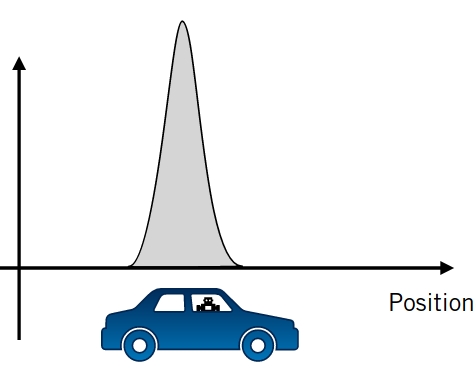
\includegraphics[width=0.8\textwidth]{./images/kalman_car.png}
                \caption{Exemplo Deslocamento Carro}
            \end{figure}
        
        Tempo contínuo
        \begin{equation*}
           \left\{
            \begin{matrix}
                s = & s_0 + vt \\
                v = & v_0 + at
            \end{matrix}, 
            \quad
            \mathbf{x} = 
            \begin{bmatrix}
                x \\
                \dot{x}
            \end{bmatrix},
            \right.
        \end{equation*}
        
        \begin{equation*}
            \text{e, }\mathbf{u}=a
        \end{equation*}

        \end{column}
        \begin{column}[c]{0.6\textwidth}
            
            \textbf{Eq. Movimento - Tempo Discreto}:

            \begin{equation*}
                \mathbf{x}_t = 
                \begin{bmatrix}
                        1 & \Delta t \\
                        0 & 1
                \end{bmatrix}
                \mathbf{x}_{t-1} +
                \begin{bmatrix}
                        0 \\
                        \Delta t
                \end{bmatrix}
                \mathbf{u}_{t-1} +
                \mathbf{w}_{t-1}
            \end{equation*}

            \textbf{Eq. Sensor - Tempo Discreto}:

            \begin{equation*}
                \mathbf{z}_t = 
                \begin{bmatrix}
                        1 & 0
                \end{bmatrix}
                \mathbf{x}_{t} +
                v_{t}
            \end{equation*}            

            \textbf{Ruído}:

            $\mathbf{w}_t \sim \mathcal{N} 
                \left(
                    \begin{bmatrix}
                    0 \\ 0    
                    \end{bmatrix},
                    \begin{bmatrix}
                    0.1 & 0 \\
                    0   & 0.1
                \end{bmatrix}
                \right)$ e :
            
            $ v_t \sim \mathcal{N} (0,0.05)$

        \end{column}
    \end{columns}
\end{frame}



\begin{frame}[c]{Kalman filter}
    \framesubtitle{Exercício - Deslocamento Carro - Kalman Filter}
    
    \begin{itemize}
        \item 1) Dado o sistema que descreve o deslocamento do carro acima,
        calcule o primeiro passo do algoritmo Kalman Filter.
    \end{itemize}

    \begin{columns}
        \begin{column}[c]{0.4\textwidth}
            \begin{figure}
                \centering
                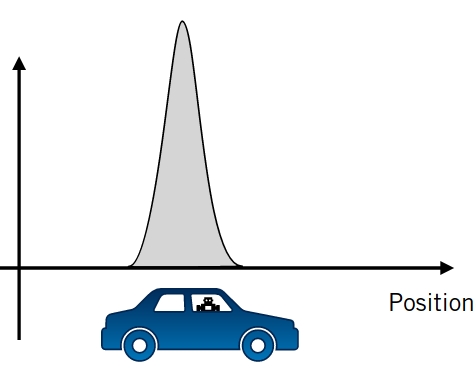
\includegraphics[width=0.8\textwidth]{./images/kalman_car.png}
                \caption{Exemplo Deslocamento Carro}
            \end{figure}
            
        \end{column}
        \begin{column}[c]{0.6\textwidth}
            
            \textbf{Condições Iniciais}:

            \begin{equation*}
                \mu_0 \sim \mathcal{N} \left( 
                    \begin{bmatrix}
                        0 \\ 5
                    \end{bmatrix}, 
                    \begin{bmatrix}
                        0.01 & 0 \\
                        0 & 1
                    \end{bmatrix} \right)
            \end{equation*}

            $\Delta t = 0.5s$

            $u_0 = -2m/s^2$

           $z_1 = 2.2 m$ 

        \end{column}
    \end{columns}
\end{frame}



\begin{frame}[c]{Extended Kalman Filter}
    \framesubtitle{Introdução}
    \begin{itemize}
        \item \textcolor{red}{Sistema do Mundo Real não são lineares};
        \item O filtro de Kalman foi desenvolvido para sistemas lineares, e normalmente assume-se que todas as perturbações e ruídos podem ser descritos com uma distribuição gaussiana de média zero;
        \item \textcolor{blue}{Se qualquer uma das transições de estado ou equações de saída do sistema for uma função não linear}, o filtro de Kalman convencional pode não mais produzir uma estimativa de estado ideal. Para contornar o problema das não linearidades, um \textcolor{blue}{Extended Kalman Filter (EKF) foi desenvolvido}, onde as não linearidades do sistema são aproximadas com modelos lineares locais;
        \item \textbf{Portanto, o algoritmo EKF é comumente usado na prática};
    \end{itemize}

\end{frame}


\begin{frame}[c]{Extended Kalman Filter}
    \framesubtitle{Introdução}
    \begin{itemize}
        \item Um exemplo clássico de sistemas considerado puramente linear é o do resistor,


    \begin{figure}
        \centering
        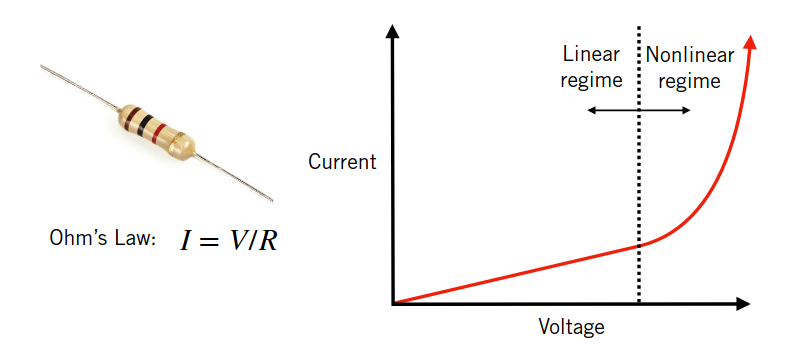
\includegraphics[width=0.8\textwidth]{./images/resistor_curve.png}
        \caption{Curva experimental de corrente vs tensão Resistor}
    \end{figure}

        \item Neste caso, o resistor tem um compartamento linear até determinada faixa de operação.
    \end{itemize}
\end{frame}


\begin{frame}[t]{Extended Kalman Filter}
    \framesubtitle{Sistemas Não Lineares}

    \begin{itemize}
        \item Problemas de Robótica Móvel mais realistas envolvem equação não lineares.
        \item Um sistema não linear pode ser escrito de uma forma geral:
        
        \begin{equation}
            \begin{split}
            x_t = & g(u_t, x_{t-1})\\
            z_t = & h(x_t)
            \end{split}
        \end{equation}
    
    onde $g(u_t, x_{t-1})$ e $h(x_t)$ são funções não lineares que representam, consecutivamente, 
    o modelo do sistema e o modelo dos sensores.

    \end{itemize}

    \begin{block}{Então como resolver esse problema?}
        \centering
        \Large{\textcolor{blue}{Linearização do Sistema}}
    \end{block}

\end{frame}

\begin{frame}[c]{Extended Kalman Filter}
    \framesubtitle{Linearização de sistemas}
    \begin{itemize}
        \item Podemos achar função linear do sistema no ponto $\color{red}{a}$ através da Expansão da Série de Taylor. Um exemplo interativo: \href{https://www.desmos.com/calculator/oiexhzavjp}{link}.

    \begin{figure}
        \centering
        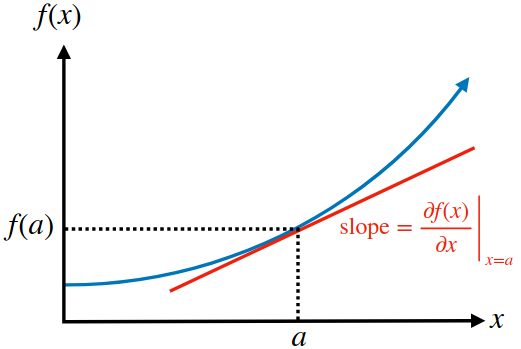
\includegraphics[width=0.4\textwidth]{./images/taylor.png}
    \end{figure}

        \begin{equation}
            f(x) = \color{red}{f(a) + \left. \frac{\partial f(x)}{\partial x} \right\vert_{x=a}(x-a)} + 
            \color{gray}{\frac{1}{2!}\left. \frac{\partial^2 f(x)}{\partial^2 x} \right\vert_{x=a}(x-a)^2 + \cdots}
        \end{equation}

        \item Para o EKF, \textcolor{red}{apenas a aproximação de primeira ordem é utilizada}.
    \end{itemize}

\end{frame}




\begin{frame}[c]{Extended Kalman Filter}
    \framesubtitle{Linearização de sistemas}
    \begin{itemize}
        \item Assim, aplicando ao sistema de equações temos:
    \end{itemize}

        \begin{block}{Prediction}
            \begin{equation*}
                \begin{split}
                    g(u_t, x_{t-1} \approx & g(u_t, \mu_{t-1}) + \frac{\partial g(u_t, \mu_{t-1}) }{\partial x_{t-1}}(x_{t-1}-\mu_{t-1}) \\
                    g(u_t, x_{t-1} \approx & g(u_t, \mu_{t-1}) + \color{red}{G_t}\color{gray}{(x_{t-1}-\mu_{t-1})}
                \end{split}
            \end{equation*}
            onde $\color{red}G_t$ é calculado pela Matriz Jacobiana.
        \end{block}


        \begin{block}{Measurement Update}
            \begin{equation*}
                \begin{split}
                    h(x_t) \approx & h(\overline{\mu}_t) + \frac{\partial h(\overline{\mu}_t) }{\partial x_{t}}(x_{t}-\overline{\mu}_{t}) \\
                    h(x_t) \approx & h(\overline{\mu}_t) + \color{blue}{H_t}\color{gray}{(x_{t}-\overline{\mu}_{t})}
                \end{split}
            \end{equation*}
            onde $\color{blue}H_t$ é calculado pela Matriz Jacobiana.
        \end{block}

\end{frame}

\begin{frame}[c]{Extended Kalman Filter}
    \framesubtitle{Linearização de sistemas}

    \begin{itemize}
        \item A matrix Jacobiana é data por:

        \begin{equation*}
        \mathbb{J}
        =
        \frac{d \mathbf{f}}{d \mathbf{x}}
        =
        \left[ \frac{\partial \mathbf{f}}{\partial q_1}
            \cdots \frac{\partial \mathbf{f}}{\partial x_n} \right]
        =
        \begin{bmatrix}
            \frac{\partial f_1}{\partial x_1} & \cdots &
            \frac{\partial f_1}{\partial x_n}                   \\
            \vdots                            & \ddots & \vdots \\
            \frac{\partial f_m}{\partial x_1} & \cdots &
            \frac{\partial f_m}{\partial x_n}
        \end{bmatrix}
    \end{equation*}
    \end{itemize}


    \begin{block}{Exemplo}
        dado um sistema representado por $\mathbf{F(x)}$, calcule a
    matriz jacobina do sistema:
    
    \begin{equation*}
        \mathbf{F(x)}
        =
        \begin{bmatrix}
            f_1 \\
            f_2
        \end{bmatrix}
        =
        \begin{bmatrix}
            x_1 + x_2 \\
            x_1^2
        \end{bmatrix}
    \end{equation*}
    
    logo:

    \begin{equation*}
        \frac{d \mathbf{f(x)}}{d \mathbf{x}}
        =
        \begin{bmatrix}
            \frac{\partial f_1}{\partial x_1} &
            \frac{\partial f_1}{\partial x_2} \\
            \frac{\partial f_2}{\partial x_1} &
            \frac{\partial f_2}{\partial x_2}
        \end{bmatrix}
        =
        \begin{bmatrix}
            1 & 1 \\
            2x_1 & 0
        \end{bmatrix}
    \end{equation*}
\end{block}


\end{frame}


\begin{frame}[c]{Extended Kalman Filter}
    \framesubtitle{Algoritmo}
    \begin{algorithm}[H]
        \caption{Extended-Kalman-Filter}
        \label{array-sum}
        \begin{algorithmic}[1]
        \Procedure{Prediction}{$\mu_{t-1}, {\textstyle\sum}_{t-1}, u_t$}
            \State $\overline{\mu}_t = g(u_t, \mu_{t-1})$
            \State $ \overline{\textstyle\sum}_t = G_t {\textstyle\sum}_{t-1} G_t^T+ Q_t$ 
            \State \textbf{Return} $\left(\overline{\mu}_t, \overline{\textstyle\sum}_t\right)$
        \EndProcedure
        \Procedure{Update}{$\overline{\mu}_{t}, \overline{\textstyle\sum}_{t}, z_t$}
            \State $K_t = \overline{\textstyle\sum}_tH_t^T(H_t\overline{\textstyle\sum}_tH_t^T+R_t)^{-1}$
            \State $\mu_t  = \overline{\mu}_t + K_t(z_t -h(\overline\mu_t))$
            \State{$\textstyle\sum_t = (I-K_t H_t)\overline{\textstyle\sum}_t$}
            \State \textbf{Return} $\left(\mu_t, \textstyle\sum_t\right)$
        \EndProcedure
        \end{algorithmic}
    \end{algorithm}
\end{frame}


\begin{frame}[c]{Extended Kalman filter}
    \framesubtitle{Exercício - Deslocamento Carro - Extended Kalman Filter}    \begin{columns}
        \begin{column}[c]{0.4\textwidth}
            \begin{figure}
                \centering
                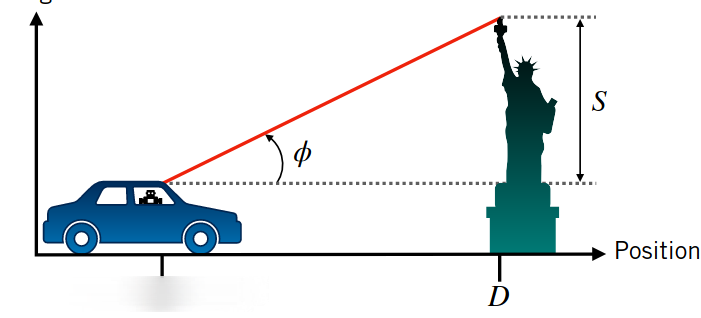
\includegraphics[width=1\textwidth]{./images/kalman_car2.png}
                \caption{Exemplo Deslocamento Carro}
            \end{figure}
        
        Tempo contínuo
        \begin{equation*}
           \left\{
            \begin{matrix}
                s = & s_0 + vt \\
                v = & v_0 + at
            \end{matrix}, 
            \quad
            \mathbf{x} = 
            \begin{bmatrix}
                x \\
                \dot{x}
            \end{bmatrix},
            \right.
        \end{equation*}
        
        \begin{equation*}
            \text{e, }\mathbf{u}=a
        \end{equation*}

        \end{column}
        \begin{column}[c]{0.6\textwidth}
            
            \textbf{Eq. Movimento - Tempo Discreto}:

            \begin{equation*}
                \mathbf{x}_t = 
                \begin{bmatrix}
                        1 & \Delta t \\
                        0 & 1
                \end{bmatrix}
                \mathbf{x}_{t-1} +
                \begin{bmatrix}
                        0 \\
                        \Delta t
                \end{bmatrix}
                \mathbf{u}_{t-1} +
                \mathbf{w}_{t-1}
            \end{equation*}

            \textbf{Eq. Sensor - Tempo Discreto}:

            \begin{equation*}
                \mathbf{z}_t = \phi_t  = 
                \tan^{-1}\left(\frac{S}{D-x_t} \right) +
                v_{t}
            \end{equation*}            

            \textbf{Ruído}:

            $\mathbf{w}_t \sim \mathcal{N} 
                \left(
                    \begin{bmatrix}
                    0 \\ 0    
                    \end{bmatrix},
                    \begin{bmatrix}
                    0.1 & 0 \\
                    0   & 0.1
                \end{bmatrix}
                \right)$ e :
            
            $ v_t \sim \mathcal{N} (0,0.05)$

        \end{column}
    \end{columns}
\end{frame}



\begin{frame}[c]{Extended Kalman filter}
    \framesubtitle{Exercício - Deslocamento Carro - Extended Kalman Filter}
    
    \begin{itemize}
        \item 1) Dado o sistema que descreve o deslocamento do carro acima,
        calcule o primeiro passo do algoritmo Extended Kalman Filter.
    \end{itemize}

    \begin{columns}
        \begin{column}[c]{0.4\textwidth}
            \begin{figure}
                \centering
                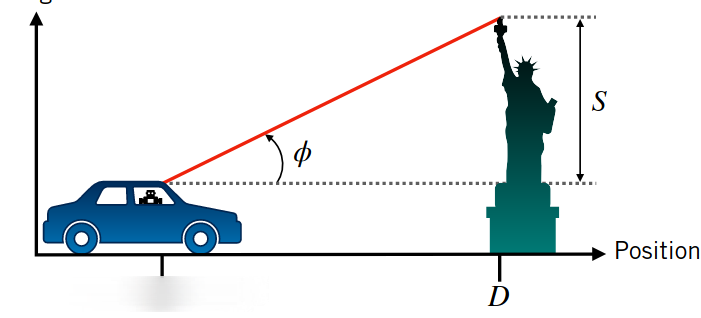
\includegraphics[width=1\textwidth]{./images/kalman_car2.png}
                \caption{Exemplo Deslocamento Carro}
            \end{figure}
            
        \end{column}
        \begin{column}[c]{0.6\textwidth}
            
            \textbf{Condições Iniciais}:

            \begin{equation*}
                \mu_0 \sim \mathcal{N} \left( 
                    \begin{bmatrix}
                        0 \\ 5
                    \end{bmatrix}, 
                    \begin{bmatrix}
                        0.01 & 0 \\
                        0 & 1
                    \end{bmatrix} \right)
            \end{equation*}

            $\Delta t = 0.5s$

            $u_0 = -2m/s^2$

           $z_1 = \frac{\pi}{6} rad$ 

           $D = 40m$

           $S = 20m$

        \end{column}
    \end{columns}
\end{frame}



\begin{frame}[t]{Referências}

    \begin{itemize}
        \item Sebastian Thrun, Wolfram Burgard, Dieter Fox. Probabilistic Robotics (Intelligent Robotics and Autonomous Agents series). The MIT Press, 2005.
        \item Roland Siegwart, Illah Reza Nourbakhsh, Davide Scaramuzza. Introduction to Autonomous Mobile Robots (Intelligent Robotics and Autonomous Agents series), 2nd ed. The MIT Press, 2011.
    \end{itemize}

\end{frame}
\end{document}



% % https://classroom.udacity.com/courses/ud810/